 \documentclass[12pt]{article}
\setlength{\columnsep}{18pt}
\usepackage[margin=1in]{geometry}
\usepackage[T1]{fontenc}
\usepackage{lmodern}
\usepackage{microtype}
\usepackage{amsmath,amssymb,amsfonts}
\usepackage{bm}
\usepackage{amsthm}
\theoremstyle{remark}
\newtheorem*{remark}{Remark}
\usepackage{siunitx}
\sisetup{detect-all,per-mode=symbol}
\usepackage{graphicx}
\usepackage{float}
\usepackage{dblfloatfix}
\graphicspath{{figures/}{Plots/}}
\usepackage{booktabs}
\usepackage{multirow}
\usepackage{caption}
\captionsetup[figure]{font=small, labelfont=bf}
\usepackage{subcaption}
\usepackage[
  style=chem-acs,
  sorting=none,
  articletitle=true,
  doi=true,
  url=true,
  maxbibnames=99,
  backend=biber
]{biblatex}
\addbibresource{references.bib}
\renewcommand*{\bibfont}{\small}
\usepackage[colorlinks=true,linkcolor=black,citecolor=black,urlcolor=black]{hyperref}
\usepackage[capitalize,noabbrev,nameinlink]{cleveref}
\usepackage{titling}
\setlength{\droptitle}{-5.5em}
\usepackage{mfirstuc}
\MakeRobust{\capitalisewords}
\MFUhyphentrue
\usepackage{subfiles}
\usepackage{authblk}
\setcounter{Maxaffil}{0}
\renewcommand\Affilfont{\itshape\small}
\renewcommand\Authfont{\normalsize}
\renewcommand\Authsep{, }
\renewcommand\Authands{ and }
\newcommand{\secref}[1]{\Cref{#1} (\nameref{#1})}
% CUSTOM COMMANDS & Formatting
\newcommand{\pmtt}{\textrm{PM\textsubscript{2.5}}}
\newcommand{\units}{\si{\micro\gram\per\cubic\meter}}
\newcommand{\city}[1]{\capitalisewords{\MakeLowercase{#1}}}
% Metrics
\newcommand{\MAPE}{\ensuremath{\mathrm{MAPE}}}
\newcommand{\RMSE}{\ensuremath{\mathrm{RMSE}}}
\newcommand{\MAE}{\ensuremath{\mathrm{MAE}}}
% Sensor counts
\newcommand{\nLucknow}{71}
\newcommand{\nDhaka}{35}
% FLOAT PARAMETERS 
\setcounter{topnumber}{3}
\setcounter{bottomnumber}{2}
\setcounter{totalnumber}{4}
\renewcommand{\topfraction}{0.9}
\renewcommand{\bottomfraction}{0.8}
\renewcommand{\textfraction}{0.05}
\renewcommand{\floatpagefraction}{0.8}
\setlength{\textfloatsep}{10pt plus 2pt minus 2pt}
\setlength{\floatsep}{8pt plus 2pt minus 2pt}
\setlength{\intextsep}{8pt plus 2pt minus 2pt}
\setlength{\abovecaptionskip}{6pt}
\setlength{\belowcaptionskip}{0pt}

\title{How many \pmtt\ sensors are needed to estimate daily and annual deployed-network mean concentrations in city-scale sensor networks?}

%AUTHORS
\author[1,$\dagger$]{Trailokaya Raj Bajgain}
\author[1,$\dagger$]{Zachary D. Calhoun}
\author[2,3]{Sachchida Nand Tripathi}
\author[4]{Abdus Salam}
\author[2,5]{Vaishali Jain}
\author[2]{Sandeep Madhwal}
\author[6]{Shahid Uz Zaman}
\author[4,7]{Shatabdi Roy}
\author[1,$\ast$]{Michael Bergin}
\author[1,8,$\ast$]{David Carlson}
\affil[1]{Department of Civil and Environmental Engineering, Duke University, Durham, NC, USA}
\affil[2]{Department of Civil Engineering, Indian Institute of Technology Kanpur, Kanpur, India}
\affil[3]{Kotak School of Sustainability, Indian Institute of Technology Kanpur, Kanpur, India}
\affil[4]{Department of Chemistry, Faculty of Science, University of Dhaka, Dhaka, Bangladesh}
\affil[5]{Atmospheric Chemistry, Max Planck Institute for Chemistry, Mainz, Germany}
\affil[6]{Department of Chemistry, Faculty of Science, Bangladesh University of Engineering and Technology, Dhaka, Bangladesh}
\affil[7]{Department of Chemistry, University of Michigan, Ann Arbor, MI, USA}
\affil[8]{Department of Biostatistics and Bioinformatics, Duke University, Durham, NC, USA}


% ACS latex guide suggests using date for e-mail
\date{Correspondence: david.carlson@duke.edu, michael.bergin@duke.edu}  

\begin{document}
\maketitle
% Template recommends using asterisk for corresponding authors
\begingroup
\renewcommand\thefootnote{\fnsymbol{footnote}}
\footnotetext[2]{Denotes equal contribution.}
\footnotetext[1]{Corresponding authors.}
\endgroup
%Abstract
\begin{abstract}
\noindent

Low-cost \pmtt\ sensor networks can increase the spatial and temporal resolution of ambient \pmtt\ monitoring. The number of sites needed for a network depends on the estimand. We quantify how closely smaller subnetworks reproduce daily and annual means of the complete deployed networks. We analyzed Dhaka, Bangladesh ($N=\nDhaka$; annual mean $55.15~\units$), Lucknow, India ($N=\nLucknow$; $61.80~\units$), and a nine-month Open Air Chicago Network ($N=277$; period mean $10.25~\units$). For each subnetwork size $n$, $10{,}000$ simple-random subnetworks were drawn without replacement and compared with the mean of the deployed-network. For annual means in Dhaka/Lucknow and the Chicago period mean, median absolute percentage error (MdAPE; typical-case) at $n=10$ was $3.9\%$, $5.6\%$, and $1.9\%$; 5--7 sensors met a relative standard error (RSE; variance-sensitive) criterion of $<10\%$ in the two full-year South Asian networks. For daily means, $n=10$ gave typical-day MdAPE of $2.6$--$5.8\%$, whereas high-variance days and the RSE criterion required roughly 30--40 sensors. In Chicago, calibration shifted the period mean by ${\sim}40\%$ ($17.18$ to $10.25~\units$) yet the relative error changed minimally at $n=10$ (MdAPE $2.8\%$ vs $1.9\%$). 10--15 spatially distributed sensors captured most of the annual-mean accuracy; neighborhood gradients, hotspots, exceedance classification, and population exposure likely require different designs.

\end{abstract}

\section*{Keywords}
{low-cost sensor networks; \pmtt\ monitoring; \pmtt\ network design; optimal sensor placement}


\section*{Synopsis}
For deployed-network mean estimation, calibrated low-cost \pmtt\ sensor subnetworks can approximate larger-network daily and annual means, informing sensor-count decisions in resource-constrained monitoring programs.



\textit{Alternative: }Monte Carlo subsampling of calibrated PM$_{2.5}$ sensor networks in Dhaka, Lucknow, and Chicago quantifies how sensor count affects estimates of deployed-network daily and annual means.




% Introduction
\section*{Introduction}\addcontentsline{toc}{section}{Introduction}\label{sec:intro}

Low-cost sensors are expanding \pmtt\ monitoring by enabling denser networks of observations. However, lower material costs do not imply lower costs overall; maintenance and overhead often dominate network costs over time.\supercite{kumar_2015_RiseLowcostSensing} In resource-constrained settings, monitoring projects still face an important optimization problem: what is the fewest number of low-cost sensors required to estimate a clearly defined network-level mean concentration target? In this manuscript, we consider the minimum network size needed to estimate daily and annual means across deployed monitoring locations, averaging periods relevant to regulatory and epidemiological contexts.\supercite{noauthor_who_2021,us_epa_national_2020}

Regulatory monitoring networks are based on Federal Reference Methods (FRM) and Federal Equivalent Methods (FEM) instruments. These instruments, based on rigorous standards for accuracy and precision, can produce very high-quality data for regulatory applications and are the only methods allowed to evaluate regulatory compliance in the USA.\supercite{us_epa_40cfr_58_app_c} However, their operational complexity and high cost have traditionally limited them to sparse networks paired with model-based spatial interpolation (e.g., kriging, land-use regression, or chemical transport modeling), often optimized for hotspot detection, compliance assessment, or exposure gradient estimation. With low-cost sensor networks, the pool of potential locations and the number of sensors can be much larger, though the required network design and size ultimately depend on the monitoring goal. For the specific goal of estimating deployed-network means, however, there is limited empirical guidance on how network size alone affects accuracy.

This lack of empirical guidance is a recognized gap in the literature. A 2023 review of long-term low-cost sensor campaigns by Carotenuto et al. highlights that protocols defining the optimal number of nodes for sufficient coverage are ``still missing,'' and nearly half (46.8\%) of reviewed real-world networks consist of only 3–10 stations.\supercite{carotenuto_low-cost_2023} Validating whether such ``small-$n$'' networks are scientifically viable for specific monitoring objectives is critical for evaluating a large portion of the current global monitoring infrastructure. Dense sensor networks have their own importance and they have enabled us to answer research questions that were previously difficult to address using the sparse FRM/FEM network. Their applications range from mapping neighborhood-level air quality and supporting exposure-gradient analyses to newer data-intensive approaches such as training AI models on high-resolution satellite image data and dense sensor networks to help predict \pmtt\ and detect hotspots in a city. However, if the target is the daily or annual mean across an existing deployed network, a smaller number of well-sited sensors may suffice. 

The emergence of low-cost sensor networks and their ability to add greater spatial coverage to air quality monitoring now makes it possible to estimate the number of sensors needed to estimate network-level temporal mean concentrations with a desired error. With this in mind, our analysis targets two statistics with distinct sampling demands: annual means, which benefit from temporal aggregation and typically stabilize with fewer independent sensors, and daily means, which remain sensitive to short-lived spatial heterogeneity from traffic, boundary-layer dynamics, and local, regional or episodic sources. We focus explicitly on mean concentrations across the deployed sensor locations at daily and annual scales, and not on estimating a true city-wide or population-weighted exposure mean, regulatory compliance, extremes, intra-urban gradients, or individual exposure. We used one year of high-fidelity (i.e., calibrated and harmonized) observations from dense low-cost \pmtt\ networks in \city{Lucknow}, India, and \city{Dhaka}, Bangladesh, collected with identical hardware and common Quality Assurance/Quality Control (QA/QC) workflows,\supercite{tsi_bluesky_2020,madhwal_evaluation_2024,jain_hybrid_2024,zaman_comparison_2025,saeed_sustaining_2025} and we include nine months of complementary data from the Open Air Chicago program as a lower-concentration developed-world transferability case. For each statistic, we evaluate the number of sensors needed to attain a desired precision under normal and lognormal distributional assumptions. We then consider whether the presence of spatial autocorrelation allows for higher-efficiency mean estimators, which would enable lower variance estimates with fewer sensors. Lastly, we use Monte Carlo simulation to analyze the bias, coverage, and error of network sub-sample estimates (of varying size $n$) with respect to the network population estimate (of size $N$) under both normal and lognormal assumptions. To help network designers achieve maximum independence and prevent biased estimates in their data, we also summarize evaluation metrics for comparing sets of potential sensor locations so that the set can be chosen that is optimally balanced over the area of interest.

\section*{Materials and Methods}\addcontentsline{toc}{section}{Materials and Methods} \label{sec:methods}
\setcounter{section}{2}
\subsection{Data}
\subsubsection{Study Areas and Networks}\label{sec:networks}
We use \pmtt\ data from three urban sensor networks. The two primary networks --- in \city{Lucknow}, India, and \city{Dhaka}, Bangladesh --- are part of a multi-country air-quality capacity-building initiative that deployed approximately 380 low-cost sensors (LCS) across South Asia, including 75 in Bangladesh and 71 in India, with additional networks in Pakistan, Sri Lanka, Nepal, the Maldives, and Bhutan.\supercite{saeed_sustaining_2025} The deployment teams are co-authors of this manuscript, supporting the high-fidelity treatment of the data described in Section~\ref{sec:qaqc}. Both use identical hardware: the {TSI BlueSky 8143} monitor with a {Sensirion SPS30} optical particle counter.\supercite{jain_hybrid_2024,zaman_comparison_2025} The third network, in \city{Chicago}, USA, is drawn from the Open Air Chicago program and is included as a partial-year transferability case in a lower-concentration developed-world setting with co-located EPA AQS reference monitors. Comparative network properties are summarized in Table~\ref{tab:spatial_support}.

\paragraph{\city{Lucknow}, India.} Lucknow, the capital of Uttar Pradesh, lies in the central Indo-Gangetic Plain (IGP), with no significant topographic relief that would create persistent meteorological boundaries. Lucknow district covers $2{,}528~\mathrm{km}^2$ and had a population of about 4.6 million in the 2011 census (2023 projection: 5.7 million).\supercite{madhwal_evaluation_2024} Its air quality is shaped by a combination of strong local emissions --- traffic, construction dust, residential cooking, and brick kilns --- alongside regional transport, especially during stagnant post-monsoon and winter periods.\supercite{madhwal_evaluation_2024,jain_hybrid_2024} Our analysis uses the dense SAAQM (Sensor-Based Ambient Air Quality Monitoring) network of {\nLucknow} sensors distributed across the district footprint in a mix of urban and peri-urban contexts, as described in Madhwal et al.\ and Jain et al.\supercite{madhwal_evaluation_2024, jain_hybrid_2024} The network was operated with collaboration at IIT Kanpur, with maintenance and calibration described in Section~\ref{sec:qaqc}. Figure~\ref{fig:sensor_networks} shows the spatial footprint of this network, which covers almost the entire district and spans a convex-hull area of $1{,}505~\mathrm{km}^2$. Here and elsewhere, we use the convex hull of the sensor locations --- the smallest convex polygon containing all sensors --- as a transparent description of the spatial extent over which network-mean estimates are defined; it is not equivalent to the administrative district area or to a population-weighted exposure footprint.

\begin{table}[t]
\centering
\small
\caption{Spatial support of the three reference networks. Network area is the convex hull of sensor locations; administrative area is provided for context but is not the estimation target. Density and pairwise distances describe the realized spatial sampling. For Chicago, the primary network excludes nine sensors collocated with EPA AQS regulatory sites.}
\label{tab:spatial_support}
\resizebox{\textwidth}{!}{%
\begin{tabular}{lrrr}
\toprule
 & \textbf{Lucknow} & \textbf{Dhaka} & \textbf{Chicago} \\
\midrule
Sensors in finite population ($N$) & 71 & 35 & 277 \\
Convex-hull area (km$^2$) & 1{,}505 & 343 & 696 \\
Administrative area (km$^2$) & 2{,}528 (district) & 2{,}570 (metro) & 606 (city) / 4{,}235 (county) \\
Sensor density (per 100 km$^2$ hull) & 4.7 & 10.2 & 39.8 \\
Median pairwise distance (km) & 13.1 & 7.9 & 13.9 \\
Median nearest-neighbor (km) & 1.9 & 1.6 & 1.4 \\
Study window & Apr 2022 -- Mar 2023 & Apr 2022 -- Mar 2023 & Sep 2025 -- May 2026 \\
Window length & 12 months & 12 months & 9 months \\
Estimation target & Deployed LCS mean & Deployed LCS mean & Deployed LCS mean \\
Reference monitor context & CAAQM (regional) & U.S.\ Embassy BAM & 10 EPA AQS sites \\
\bottomrule
\end{tabular}}
\end{table}


\paragraph{\city{Dhaka}, Bangladesh.} Dhaka, the capital of Bangladesh, lies in the lower IGP delta. The terrain is low-lying delta with no significant topographic relief, but with a dense river network that influences local boundary-layer behavior. The Dhaka Metropolitan Area spans $2{,}570~\mathrm{km}^2$ and had a population of about 21.6 million as of the 2022 census, while Dhaka City had roughly 10.3 million residents.\supercite{noauthor_population_2022} Its extreme population density and rapid urban expansion create a complex urban airshed dominated by local emissions from brick kilns, vehicular traffic, industrial activities, and biomass burning, compounded by regional transboundary transport and strong monsoon--winter seasonality.\supercite{zaman_comparison_2025} The Dhaka network of {\nDhaka} sensors is operated jointly by collaborators at the University of Dhaka and Bangladesh University of Engineering and Technology, with maintenance and calibration described in Section~\ref{sec:qaqc}. Sensor siting is concentrated in the urban core to support neighborhood-level studies; one peri-urban site lies outside the municipal boundary at approximately $23.6^\circ$N, $90.5^\circ$E in the Narayanganj suburb to extend coverage into a known industrial corridor. Following the same convex-hull definition above, the network spans approximately $343~\mathrm{km}^2$.

\paragraph{\city{Chicago}, USA.} Chicago is a flat lakeside metropolis on Lake Michigan in the U.S.\ Midwest, with no significant topographic relief that would create persistent meteorological boundaries. The City of Chicago covers $606~\mathrm{km}^2$ (Cook County: $4{,}235~\mathrm{km}^2$); the 2022 American Community Survey estimates 2.66 million residents within the city and 5.2 million in Cook County. The airshed is shaped by long-range transport, lake-effect meteorology, automotive emissions, and industrial activity, with annual \pmtt\ levels roughly an order of magnitude below those in \city{Lucknow} and \city{Dhaka}. Our analysis uses the Open Air Chicago low-cost sensor network of 286 calibrated LCS units; we exclude 9 sensors collocated with regulatory monitoring sites, leaving a primary finite-population network of 277 sensors. Chicago hardware is more heterogeneous than the TSI BlueSky 8143 used in South Asia, and the deployment-team calibration pipeline (against EPA AQS reference monitors) is summarized in Supporting Information~\ref{sec:si_diagnostics}. Ten EPA AQS regulatory \pmtt\ sites within Cook County provide context for instrument-level comparison but are not the estimation target. The Chicago study window spans September~1, 2025 through May~31, 2026 (nine months), so all Chicago period-mean results should be read as a partial-year transferability case and an upper bound on what a full-year analysis would yield. Chicago is included because it offers a lower-concentration developed-world counterpoint to the South Asian networks and supports transferability claims that would otherwise rest on two highly polluted cities alone; full-year quantitative recommendations, however, are presented only for \city{Lucknow} and \city{Dhaka}.

\begin{figure}[H]
    \centering
    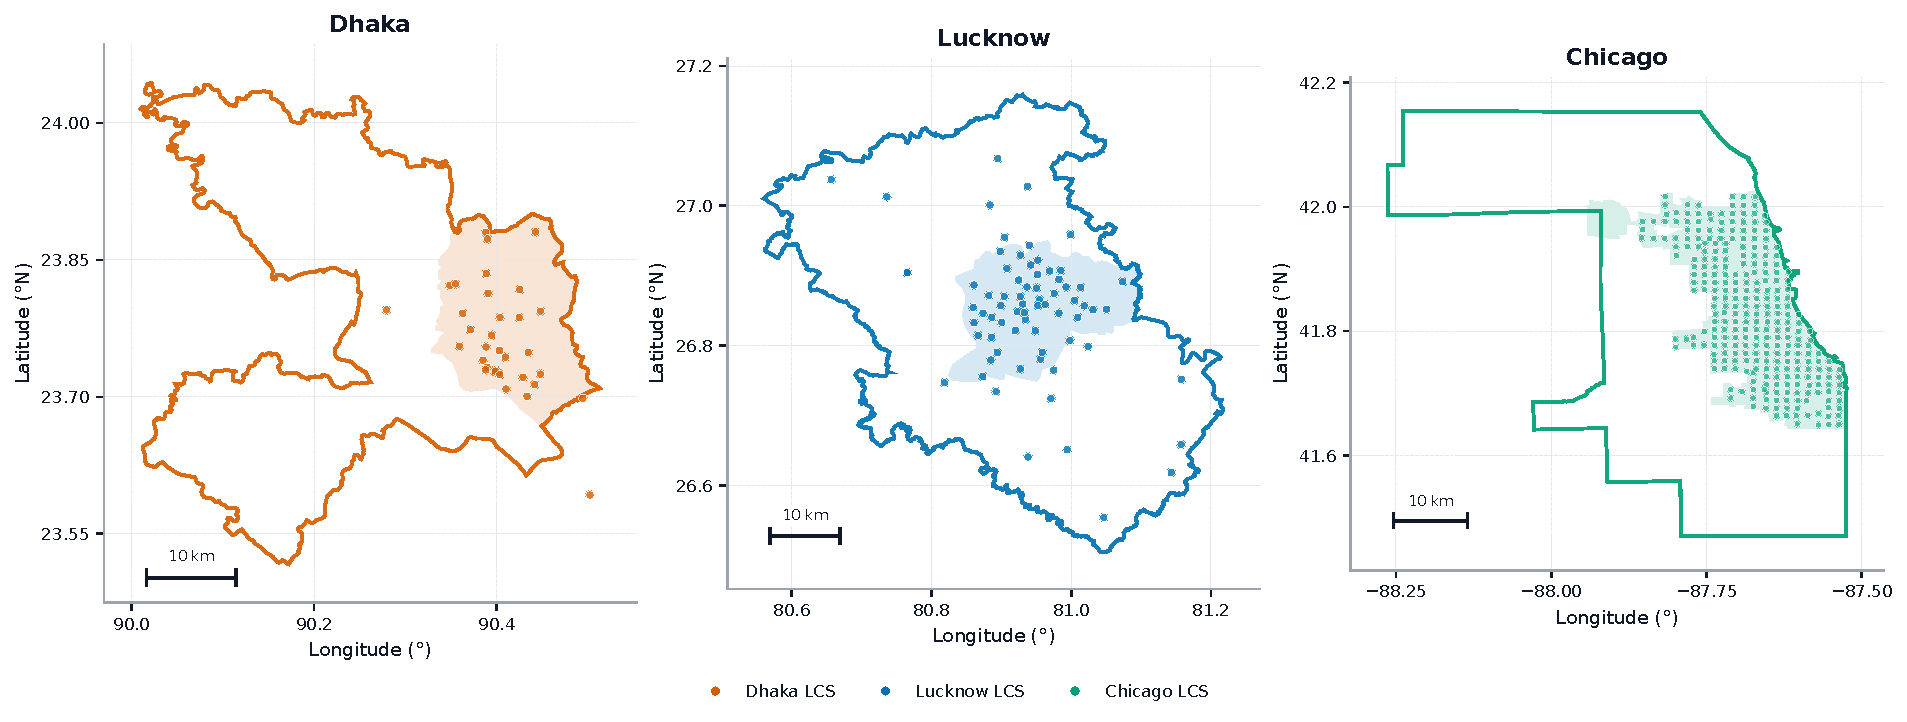
\includegraphics[width=0.95\textwidth]{Plots/Main_text/Figure_1/three_city_sensor_network_reference_monitor_map.pdf}
    \caption{Sensor networks in \city{Dhaka}, \city{Lucknow}, and \city{Chicago}. Points show low-cost sensor locations only; shaded and outlined regions denote municipal and district/county boundaries using the same city color as the sensors. Chicago EPA AQS regulatory monitors are retained as Supporting Information context and are not part of the primary low-cost-sensor finite population used for Monte Carlo subsampling.}
    \label{fig:sensor_networks}
\end{figure}



\subsubsection{Data Processing and QA/QC}\label{sec:qaqc}

\paragraph{South Asian networks.} We analyze daily and annual \pmtt\ data aggregated from hourly observations collected between April~2022 and March~2023. Both South Asian networks were deployed, maintained, and calibrated in \city{Lucknow} and \city{Dhaka}, and the data used in this study reflect the processed outputs of the established QA/QC and calibration workflows implemented by the deployment teams.\supercite{jain_hybrid_2024, madhwal_evaluation_2024, zaman_comparison_2025, shrestha_field_2025} The TSI BlueSky 8143 system reports manufacturer-corrected hourly PM concentrations from the embedded Sensirion SPS30 (which includes on-device humidity compensation), along with nowcast and 24-hour rolling values; we use the cleaned hourly \pmtt\ stream as our primary observational unit. As part of these workflows, raw measurements were automatically cleaned to remove erroneous records, flagged values, and physically implausible observations. Examples include sensor-specific error flags (``PM Sensor Error,'' ``Timestamp Stale'') and exclusion of physically implausible values such as \pmtt\ $\le 0$ or $\ge 2000$~\units. The $2000~\units$ upper threshold corresponds to clearly aphysical excursions attributable to sensor saturation or transient electronic faults rather than real ambient values; the $\le 0$ lower threshold is similarly aphysical for ambient PM. Low-but-nonzero outliers (values that are physically plausible at the instrument but anomalously low for a given location relative to its neighbors) were not retroactively removed; a diagnostic screening of low-tail values is reported in Supporting Information~\ref{sec:si_diagnostics}. After this screening, no nonphysical values remained in the processed hourly dataset, and 14.2\% (Dhaka) and 28.3\% (Lucknow) of potential hourly records were excluded post-QA/QC. We did not impose any additional completeness threshold (e.g., minimum hours per day) beyond the QA/QC flags and physical plausibility screening; sensitivity of the main conclusions to completeness thresholds is reported in Supporting Information~\ref{sec:si_diagnostics}. \city{Lucknow}'s higher missingness reflects staggered deployment in 2022 and intermittent power and connectivity outages rather than concentration-correlated dropout; supplementary screens show that day-to-day missingness is not strongly correlated with concentration level or with cross-sensor spatial variability (Supporting Information~\ref{sec:si_diagnostics}).

Calibration and harmonization were then applied by the deployment teams to align sensors both against reference-grade instruments and within-network agreement. In \city{Lucknow}, pre-deployment collocation at IIT Kanpur and in-field collocation with continuous ambient air quality monitoring (CAAQM) reference monitors provided seasonal inter-sensor and intra-sensor adjustment factors.\supercite{jain_hybrid_2024} In \city{Dhaka}, collocation against the U.S.\ Embassy BAM informed multiplicative correction factors estimated via linear regression against the network median.\supercite{zaman_comparison_2025} These calibration and harmonization factors were applied to the cleaned raw data before aggregation into the final hourly measurements. The within-batch sensor-to-sensor coefficient of variation at co-located conditions is approximately $5$--$8\%$ for the TSI BlueSky 8143 family and $7$--$10\%$ for the Sensirion SPS30 family,\supercite{jain_hybrid_2024,zaman_comparison_2025} which is smaller than the day-to-day cross-sensor coefficient of variation we observe in deployed conditions, indicating that the field heterogeneity we analyze is dominated by site-to-site differences rather than by intrinsic unit-to-unit variability. These procedures provide confidence in the reliability and consistency of the networks. We term these systems high-fidelity, well-calibrated networks; we do not claim that they are equivalent to FRM/FEM regulatory monitors, and our results should not be interpreted as a substitute for regulatory-grade compliance monitoring (see Section~\ref{sec:assumptions}).

\paragraph{Chicago network.} For Chicago we apply the same finite-population framework to the Open Air Chicago network. The official daily aggregates we use (calibrated \pmtt) reflect the program's deployed calibration pipeline, including manufacturer-side preprocessing of the heterogeneous hardware and a within-program harmonization step against EPA AQS reference monitors. The Chicago program collocates nine of its 286 LCS units at three EPA AQS reference sites for ongoing calibration verification; as noted in Section~\ref{sec:networks}, these collocated units are excluded from the primary finite population to avoid distorting the design-based sampling, leaving 277 city sensors. One Chicago daily aggregate (April~14, 2026) is missing from the official daily file due to an upstream aggregation gap in the program's reporting; we exclude that date from daily analyses. A raw versus calibrated sensitivity analysis and an LCS-vs-AQS instrument comparison are reported in Supporting Information~\ref{sec:si_diagnostics}.

\paragraph{Post-QA/QC diagnostics.} We conducted post-QA/QC diagnostics on the processed hourly dataset to characterize within-network consistency, spatial coverage over the deployed-network footprint (radial extent $\sim$0.6--21~km in Dhaka and $\sim$0.5--78~km in Lucknow), and temporal completeness (Supporting Information~\ref{sec:si_diagnostics}). After QA/QC, 85.8\% and 71.7\% of possible hourly records were retained in \city{Dhaka} and \city{Lucknow}, respectively, with median sensor uptime of 87.6\% in Dhaka and 73.2\% in Lucknow. We report median uptime rather than mean because the median is robust to a small number of sensors with very low uptime (e.g., the lowest-coverage \city{Lucknow} sensor reports 4.5\% uptime; see Supporting Information~\ref{sec:si_diagnostics}). Within-network consistency was high, with median sensor-to-network correlation $r=0.891$ in Dhaka and $r=0.950$ in Lucknow (hourly sensor series correlated against the contemporaneous network median), supporting the treatment of each reference network as the finite population for subnetwork experiments. Comparable Chicago diagnostics, including retention rates and within-network correlations, are reported in Supporting Information~\ref{sec:si_diagnostics}.

\subsubsection{Reference Mean Definitions}\label{sec:ref_mean}
We define $N$ as the number of sensors in the reference network (the finite population), and let each hourly timestamp $t$ index a unique date--hour. Reference means are computed at daily and annual scales using a two-step aggregation procedure. For \city{Lucknow} and \city{Dhaka}, ``annual'' refers to the full twelve-month deployment year (April~2022--March~2023). The \city{Chicago} deployment window spans September~1,~2025--May~31,~2026 (nine months); we therefore treat \city{Chicago} throughout as a partial-year transferability case rather than an annual mean, and reserve the term ``annual'' for the twelve-month South Asian networks.

\textbf{Temporal aggregation (sensor-level).}
For each sensor $i$, $H_i$ denotes the number of valid hourly observations within the temporal window. The sensor-level mean is
\begin{equation}\label{eq:mu_sensor}
\mu_{i} = \frac{1}{H_i} \sum_{t} y_{i,t}
\end{equation}
with the sum taken over all timestamps $t$ for which sensor $i$ reports valid data. For the \emph{daily mean} $\mu_{i,d}^{\mathrm{daily}}$ on day $d$, $H_i \le 24$; for the annual mean $\mu_i^{\mathrm{annual}}$, $H_i \le 8{,}760$ for the South Asian networks and $H_i \le 6{,}552$ for Chicago. We do not impose a minimum-$H_i$ threshold beyond the QA/QC screening described in Section~\ref{sec:qaqc}; sensors with very few valid hours therefore contribute a noisier sensor-level mean to the spatial aggregation but are not excluded. The sensitivity of the headline results to minimum-$H_i$ thresholds is reported in Supporting Information~\ref{sec:si_diagnostics}.

\textbf{Spatial aggregation (network-level).}
Let $N^*$ denote the number of sensors with at least one valid sensor-level mean within the temporal window, so that $N^* \le N$; \emph{daily} $N^*$ is the number of sensors with valid data on a given day, and \emph{annual} $N^*$ is the number of sensors with at least one valid hour during the deployment window. The network reference mean is
\begin{equation}\label{eq:mu_ref}
\mu_{\mathrm{ref}} = \frac{1}{N^*} \sum_{i=1}^{N^*} \mu_{i},
\end{equation}
that is, an unweighted average of valid sensor-level means. We do not apply area weights, population weights, or land-use weights at this stage; this choice is discussed under Assumptions in Section~\ref{sec:assumptions}. The distribution of daily $N^*$ across the study window is reported in Supporting Information~\ref{sec:si_diagnostics}; in all evaluated subnetwork sizes ($n \in \{2, \dots, 30\}$ for the headline curves), $n \le N^*$ holds on essentially every day for \city{Lucknow} and \city{Chicago}, while \city{Dhaka} has a small number of days on which $N^*$ falls below the largest tested $n$ (we report these counts in the supplementary information and exclude any subnetwork draw for which $n > N^*$).

\subsubsection{Design-Based Monte Carlo under SRSWOR}
\label{sec:monte_carlo}

\paragraph{Intuition.} Before introducing the formal framework, it is useful to state the procedure in plain terms. For each network we ask: \emph{if we had only $n$ sensors instead of all $N$, how close would the mean of those $n$ sensors be to the mean of the full network?} We answer this by repeatedly drawing random $n$-sensor subsets from the network (without replacement, so each subset is a physically realizable smaller network), computing the subset mean, comparing it to the full-network reference mean, and tabulating the distribution of errors across subsets. Sweeping $n$ from small to large traces out an error-vs-size curve. This is a design-based view: the randomness comes from how we draw subsets, not from assumed properties of the underlying pollution field.

We employ design-based Monte Carlo simulation under simple random sampling without replacement (SRSWOR), a framework grounded in finite-population survey sampling theory.\supercite{cochran_sampling_1977,lohr_sampling_2021} The term \emph{design-based} indicates that inference relies on the known randomization distribution (SRSWOR) rather than parametric assumptions about spatial pollution patterns. We treat the observed sensor network as a finite population and draw inferences based solely on the sampling design, without requiring distributional assumptions for the underlying pollution field. In this finite set of sensors, each sensor is unique, so no subset can contain repetitions. Every possible subset configuration $c$ of size $n$ is equally likely, for any $n$ between 1 and the total number of sensors $N$ in the deployed network. Formally, $\mathcal{C}_n$ denotes the set of all possible $n$-sensor subsets drawn from the deployed network without replacement:
\begin{equation}\label{eq:SRSWOR_random_distribution}
X \sim \mathrm{Unif}(\mathcal{C}_n),
\qquad
\Pr(X = c) = \frac{1}{|\mathcal{C}_n|}
\quad \text{for all } c \in \mathcal{C}_n.
\end{equation}

The complete error distribution would require evaluating all $\binom{N}{n}$ possible sensor configurations, which quickly becomes computationally infeasible. For example, selecting subsets of size $n=5$ from networks of $N=35$ and $N=71$ yields $\binom{35}{5} \approx 3.2 \times 10^5$ and $\binom{71}{5} \approx 1.3 \times 10^7$ possible configurations, respectively. For larger subsets approaching half the network size, the combinatorial explosion is extreme: $\binom{35}{18} \approx 4.5 \times 10^9$ and $\binom{71}{36} \approx 2.2 \times 10^{20}$. We therefore employ Monte Carlo approximation, drawing $B = 10{,}000$ independent and identically distributed (i.i.d.) samples from the uniform distribution: $X_1, \dots, X_B \;\overset{\text{i.i.d.}}{\sim}\; \mathrm{Unif}(\mathcal{C}_n).$ Each configuration represents a physically realizable network where no sensor appears more than once, and the sampling mechanism corresponds to SRSWOR.

\subsubsection{Estimators and Metrics} \label{sec:estimators_metrics}
\paragraph{Overview.} We compare subnetwork means to the full network mean using two estimators (the arithmetic-mean estimator and a lognormal-back-transform estimator) and four families of metrics (the median absolute percentage error, or MdAPE, which characterizes \emph{typical} subnetwork error; tail percentiles of the absolute percentage error, which characterize \emph{worst-case} behavior; the relative standard error, or RSE, which characterizes expected error under a parametric assumption; and quantile coverage error, which checks whether nominal confidence intervals attain their stated coverage). Each metric answers a distinct question and the sensor-count recommendation it implies differs accordingly. A compact mapping from metric to question is provided in Supporting Information~\ref{sec:si_metrics}.

\paragraph{Distributional Considerations.}
\pmtt\ concentrations are typically right-skewed, particularly at high concentrations and short averaging windows, and the lognormal distribution has a long history of empirical use to describe atmospheric particle concentrations.\supercite{kahn_1973_NoteDistributionAir,ott_1990_PhysicalExplanationLognormality,andersson_2021_MechanismsLogNormala,bencala_1976_FrequencyDistributionsAir} We therefore evaluate sub-sample means using both the arithmetic-mean estimator and a lognormal estimator. To avoid confusion with the network size $N$, we refer to these by name throughout the prose, while retaining $\mathcal{N}$ and $\log\mathcal{N}$ subscripts in equations where compactness is helpful. The arithmetic-mean estimator remains a valid estimator of the mean without distributional assumptions, but small-sample uncertainty quantification (e.g., $t$-based standard errors and confidence intervals) is best calibrated when the sampling distribution of the mean is approximately normal. The lognormal estimator instead targets skewness by operating on log-transformed observations and then back-transforming to the original scale.

To assess the plausibility of these distributional approximations we used the Shapiro--Wilk test applied to the cross-sectional daily distributions across sensors (Supporting Information~\ref{sec:si_distributional} and Table~\ref{tab:shapiro}). Neither of the distributions holds universally. In \city{Lucknow}, normality is rejected on most days, whereas lognormality is rejected less frequently. In \city{Dhaka}, where fewer sensors contribute to each daily distribution, both assumptions show higher rejection rates. These results indicate that normal and lognormal models are, at best, approximations for daily spatial distributions. Our headline conclusions therefore rely on the design-based MdAPE metric (defined formally below), which characterizes sub-network performance without depending on the correctness of either distributional model; the model-based RSE results are reported as a complementary expected-error view and should be read as conditional on the assumed family.

\paragraph{Absolute Percentage Error (APE).}\label{sec:APE}
For each Monte Carlo iteration $b$ with a subset size $n$, we compute the subset mean $\widehat{\mu}^{(b)}_{n}$ and compare it to the  network reference mean $\mu_{\mathrm{ref}}$ (Eq.~\ref{eq:mu_ref}). The two estimators compute $\widehat{\mu}^{(b)}_{n}$ differently: the arithmetic-mean estimator ($\mathcal{N}$) uses the arithmetic mean of sensor-level means, $\widehat{\mu}^{(b)}_{n,\mathcal{N}} = \frac{1}{n^*}\sum_{i=1}^{n^*} \mu_i$, whereas the lognormal estimator ($\log\mathcal{N}$) operates on log-transformed observations and back-transforms via $\widehat{\mu}^{(b)}_{n,\log\mathcal{N}} = \exp(\bar{y}_{\log} + s^2_{\log}/2)$, where $\bar{y}_{\log}$ and $s^2_{\log}$ are the sample mean and variance of the logged sensor-level means. The absolute percentage error ($\mathrm{APE}_{b}$) for iteration $b$ is then
\begin{equation}\label{eq:ape}
  \mathrm{APE}_{b} = \frac{ \bigl| \widehat{\mu}^{(b)}_{n} - \mu_{\mathrm{ref}} \bigr| }
       { \mu_{\mathrm{ref}} } \times 100\%.
\end{equation}
The same construction gives an absolute concentration error in \units, $\mathrm{AE}_b = | \widehat{\mu}^{(b)}_{n} - \mu_{\mathrm{ref}} |$, which we use alongside the percentage error so that readers can interpret accuracy in policy-relevant concentration units rather than in percentages alone (Supporting Information~\ref{sec:si_metrics}). A schematic distinguishing the unobserved true field, the deployed reference network used as the estimand here, and a single random subnetwork draw is provided in Figure~\ref{fig:si_estimand_schematic}. Empirical daily cross-sensor distributions on representative low, median, and high concentration days are shown in Figure~\ref{fig:si_daily_distributions}, supporting the right-skewed character of the distributions used below.

\paragraph{Median Absolute Percentage Error (MdAPE).}\label{sec:MAPE}
This sampling procedure yields, for each subset size $n$, a complete set of $B$ APE values $\{\mathrm{APE}_b\}_{b=1}^{B}$. The median absolute percentage error for subset size $n$ is
\begin{equation}\label{eq:mape}
  \mathrm{MdAPE}(n) = \text{median}\big(\mathrm{APE}_1, \mathrm{APE}_2, \dots, \mathrm{APE}_B\big).
\end{equation}
APE distributions are right-skewed, particularly on high-variance days (we visualize this directly in Figure~\ref{fig:mdape_daily} and document the empirical APE distribution in Supporting Information~\ref{sec:si_design_based}); the median is therefore a more robust descriptor of \emph{typical} subnetwork error than the mean, which is sensitive to a small fraction of high-error draws. We additionally report the 75th, 90th, and 95th APE percentiles in the Supporting Information so that worst-case behavior --- the question of how bad a suboptimal random subnetwork can be --- is also characterized.

% Results & Discussion 
\section*{Results and Discussion}\addcontentsline{toc}{section}{Results and Discussion} \label{sec:results}
\setcounter{section}{3}
\setcounter{subsection}{0}


\subsection{Annual Median Absolute Percentage Error}\label{sec:annual}
Figure~\ref{fig:mdape_annual}a shows that the median absolute percentage error decreases rapidly with subnetwork size in all three networks. At $n=10$ sensors, MdAPE is 5.6\% in \city{Lucknow} (reference mean 61.8~\units), 3.9\% in \city{Dhaka} (reference mean 55.1~\units), and 1.9\% in the nine-month \city{Chicago} window (reference mean 10.3~\units). Doubling to $n=20$ further reduces these to 3.6\%, 2.1\%, and 1.4\% respectively. This rapid convergence is due to the smoothing effect of temporal aggregation, which suppresses short-term spatial variability over the deployment window. Part of this convergence reflects regionally coherent seasonal pollution patterns shared across sensors --- a point we examine further in Supporting Information~\ref{sec:si_diagnostics}, where between-sensor variability in annual means is decomposed --- and so the rapid annual convergence should be read as a property of the specific networks studied rather than a universal claim. In all three networks, the MdAPE is likely below 10\% with as few as 3--5 sensors (i.e., with probability $>50\%$). The 95th-percentile APE, which characterizes the suboptimal-draw tail, decreases more slowly: at $n=10$ it is 15.8\% in \city{Lucknow}, 10.9\% in \city{Dhaka}, and 6.6\% in \city{Chicago}, falling to 10.4\%, 5.9\%, and 4.6\% at $n=20$. Approximately $n=25$ is needed to bring this tail metric below 10\% in the South Asian networks. Figure~\ref{fig:si_period_error_bands} visualizes these typical and worst-case bands together for all three networks. In these worst-case draws, sensors with higher-than-average observations are disproportionately sampled. As explored in Appendix~\ref{sec:annual_mean_comparison}, these sensors exhibit larger variance in their mean estimates. If we weighted observations based on their uncertainty, we may be able to reduce the influence of outliers on the annual mean. However, such a technique would step outside the design-based simulation taken here. Figure~\ref{fig:mdape_annual}b shows the same results in absolute concentration units (\units), which preserves the policy-relevant interpretability of the errors and makes the order-of-magnitude difference in baseline \pmtt\ between \city{Chicago} and the South Asian networks visible.

\begin{figure}[h]
    \centering
    \begin{subfigure}{0.86\textwidth}
        \centering
        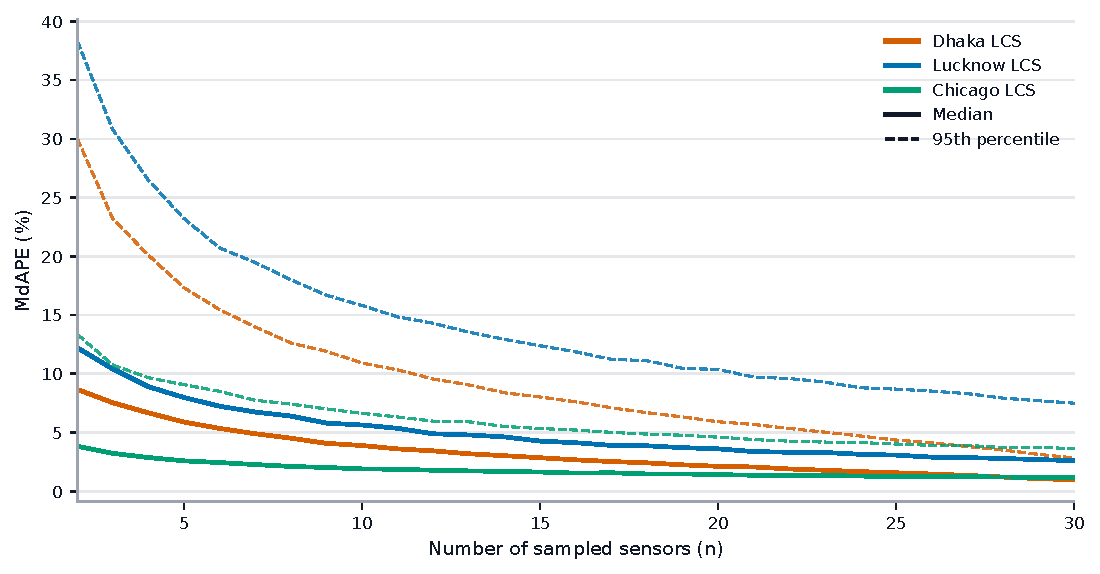
\includegraphics[width=\textwidth]{Plots/Main_text/Figure_2/period_mdape_vs_sample_size.pdf}
        \caption{Relative error}
    \end{subfigure}
    \vspace{0.3em}
    \begin{subfigure}{0.86\textwidth}
        \centering
        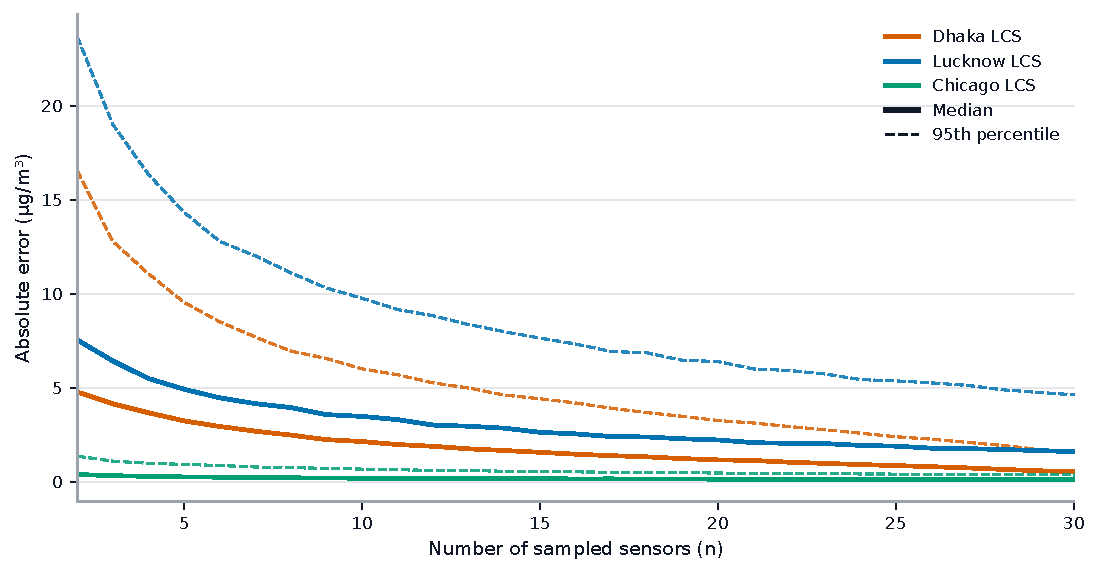
\includegraphics[width=\textwidth]{Plots/Main_text/Figure_2/period_absolute_error_vs_sample_size.pdf}
        \caption{Absolute concentration error}
    \end{subfigure}
    \caption{Absolute percentage (a) and absolute concentration (b) error for annual means as a function of subnetwork size $n$. Solid lines indicate the median across $B=10{,}000$ Monte Carlo subnetwork draws, and dashed lines indicate the 95th percentile. The Chicago curve covers a nine-month window and should be read as a partial-year case. Numerical sensor-count recommendations are reported in Section~\ref{sec:design_implications}.}
    \label{fig:mdape_annual}
\end{figure}

\subsection{Daily Median Absolute Percentage Error}\label{sec:daily}
We visualize daily MdAPE in Figure~\ref{fig:mdape_daily}. Even with 5 sensors, the across-day median daily MdAPE is 6.5\% in \city{Lucknow}, 8.8\% in \city{Dhaka}, and 3.5\% in \city{Chicago} (Supporting Information~\ref{sec:si_design_based}); MdAPE is less than 10\% on 71\% of days in \city{Dhaka} and 93\% of days in \city{Lucknow}, with a comparable high fraction in \city{Chicago}. With $n=10$ sensors, approximately 97\% of the days have $\mathrm{MdAPE}<10\%$ in \city{Dhaka} and \city{Lucknow}; the across-day median daily MdAPE at $n=10$ is 4.5\% (\city{Lucknow}), 5.8\% (\city{Dhaka}), and 2.6\% (\city{Chicago}). The worst single-draw absolute percentage error in our data at $n=10$ reaches $93\%$ in \city{Lucknow} (January~17, 2023), $88\%$ in \city{Dhaka} (May~19, 2022), and $119\%$ in \city{Chicago} (March~13, 2026), each occurring on days with anomalously elevated cross-sensor coefficient of variation; we characterize these high-error days further in Section~\ref{sec:si_high_error_days}. The daily $N^*$ trace overlaid in Figure~\ref{fig:mdape_daily} shows the number of sensors with valid data each day, contextualizing the days on which subnetwork draws of large $n$ become near-exhaustive of the available sensors.

Days with elevated MdAPE share characteristic signatures. The coefficient of variation across sensors ($\sigma/\mu$) is disproportionately high on these days, but the daily mean \pmtt\ itself is not always elevated, suggesting that high MdAPE is driven by spatial heterogeneity within the network rather than by absolute concentration level. The per-city slope of daily MdAPE at $n=10$ on daily cross-sensor coefficient of variation, reported in Supporting Information~\ref{sec:si_cv_slope}, gives a compact summary of this relationship: $\beta_{\mathrm{Dhaka}}=0.20$, $\beta_{\mathrm{Lucknow}}=0.16$, and $\beta_{\mathrm{Chicago}}=0.11$, with non-overlapping $95\%$ confidence intervals across the three cities. A regression and clustering analysis of high-error days is reported in Supporting Information~\ref{sec:si_design_based} and shows that high-error days tend to coincide with periods of high day-to-day variability, occasional anomalous sensors, and missing-data clusters rather than with a single physical mechanism. We do not interpret individual high-error days as diagnostic of specific localized sources without independent corroboration. An absolute-concentration version of Figure~\ref{fig:mdape_daily} is provided in Supporting Information~\ref{sec:si_design_based}, and a check that key diurnal and typical-day temporal features of the network signal are preserved by random subnetworks at $n \in \{5, 10, 20\}$ is reported in Supporting Information~\ref{sec:si_diagnostics}.

\begin{figure}[h]
    \centering
    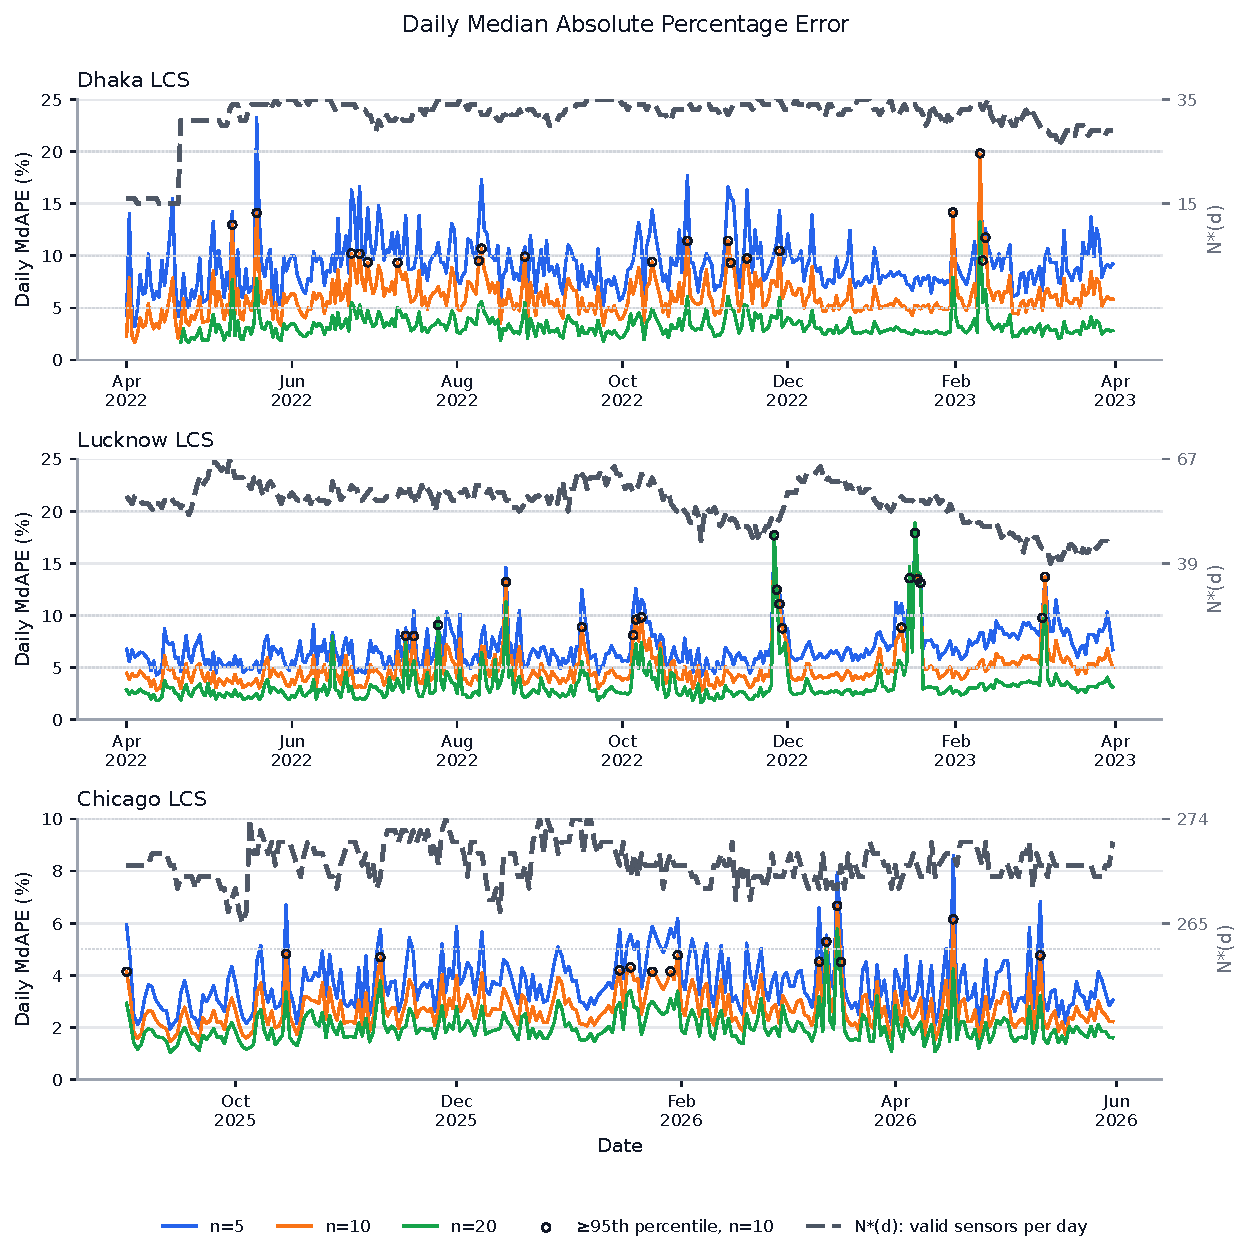
\includegraphics[width=0.98\textwidth]{Plots/Main_text/Figure_3/daily_mdape_timeseries_with_valid_sensor_count.pdf}
    \caption{Median absolute percentage error for daily mean estimates at subnetwork sizes $n\in\{5, 10, 20\}$ for \city{Dhaka}, \city{Lucknow}, and \city{Chicago} (note the \city{Chicago} panel uses a $0$--$10\%$ vertical axis, the South Asian panels a $0$--$25\%$ axis). For any given day $d$, subsets of size $n$ are drawn from the $N^*(d)$ sensors that report valid data on that day, so that $n \leq N^*(d) \leq N$, where $N$ is the full deployed-network size; sensors lacking data on a given day are excluded from that day's draws. The dashed dark-gray trace shows $N^*(d)$ compressed into the upper band of each panel (15--25\% for \city{Dhaka}/\city{Lucknow}, 6--10\% for \city{Chicago}); the secondary right-axis tick labels give the corresponding native valid-sensor counts. Open circles mark days in the upper $5\%$ of $n=10$ daily MdAPE. Results are shown for the arithmetic-mean estimator; absolute-concentration ($\mu$g\,m\textsuperscript{-3}) counterparts are provided in Supporting Information~\ref{sec:si_design_based}.}
    \label{fig:mdape_daily}
\end{figure}
\clearpage
\subsection{Estimator Bias and Coverage}\label{sec:bias_coverage}
In addition to testing the distributional assumptions, we consider whether the lognormal estimator offers any benefit over the arithmetic-mean estimator by assessing its bias and coverage. The lognormal estimator shows a small positive bias relative to the arithmetic reference mean, with the bias scaling roughly with the within-network skewness: at $n=10$ the period mean relative bias is approximately 0.10\% in \city{Chicago} (range 0.04--0.11\% across $n$), 0.41\% in \city{Dhaka} (range 0.17--0.61\%), and 0.43\% in \city{Lucknow} (range 0.24--0.90\%) (Supporting Information Figure~\ref{fig:mrb_histograms}). The bias is small relative to the typical MdAPE, and is insensitive to the number of sensors in the network --- it is a property of the estimator rather than of insufficient data. The point estimate of the MdAPE is essentially indistinguishable between the arithmetic-mean estimator and the lognormal estimator at every $n$ tested (Supporting Information~\ref{sec:si_estimator_comparison}); the difference lies in how the two estimators handle uncertainty quantification, which we examine through coverage below.

To assess statistical coverage, we calculate the quantile coverage error (QCE) over replicates for each day. This quantity is defined as the absolute value of the nominal coverage less the empirical coverage. For example, a QCE of 1\% at a nominal level of 95\% would indicate that the confidence intervals given by sub-samples contain the reference mean 94\% or 96\% of the time. We discuss this calculation in more detail in Supporting Information~\ref{sec:si_metric_definitions}. Generally, we find that the standard (arithmetic-mean, normal-theory) confidence intervals are reasonably well calibrated even at small sample sizes: across the three nominal levels the median daily quantile coverage error is within roughly 2--3 percentage points at $n \leq 10$ and tightens to within about 1 percentage point by $n=20$ (Table~\ref{tab:ci}). The lognormal estimator does not improve calibration: at the 68\% level its coverage error is larger and does not decrease appreciably with $n$ (remaining near 4--5 percentage points in \city{Dhaka}), and it is only marginally better than the normal-theory interval at the 95\% level for the smallest sample sizes. These results indicate that standard confidence-interval procedures are usable but somewhat optimistic for daily mean estimates at very small $n$; as $n$ exceeds 20 they typically attain empirical coverage within about 1 percentage point of nominal.

Together, these bias and coverage results indicate that the lognormal estimator offers no calibration advantage that would offset its positive bias for the deployed-network mean estimand considered here. We therefore retain the arithmetic-mean estimator as the default (Section~\ref{sec:design_implications}): it is unbiased for the reference mean by construction and reasonably well calibrated at the sample sizes we recommend. The lognormal estimator remains useful chiefly as a distributional diagnostic and, at the 95\% level and very small $n$, as a marginally more conservative interval.


\begin{table}[ht]
\centering
\small
\begin{tabular}{clrrrrrr}
\toprule
\textbf{City} & $n$ & \multicolumn{2}{c}{68\%} & \multicolumn{2}{c}{90\%} & \multicolumn{2}{c}{95\%} \\
\cmidrule(lr){3-4}\cmidrule(lr){5-6}\cmidrule(lr){7-8}
 &  & $\mathcal{N}$ & $\log \mathcal{N}$ & $\mathcal{N}$ & $\log \mathcal{N}$ & $\mathcal{N}$ & $\log \mathcal{N}$ \\
\midrule
\multirow{4}{*}{\city{Dhaka}} & 5 & \textbf{2.0} & 3.4 & \textbf{2.3} & 2.5 & 2.1 & \textbf{1.9} \\
 & 10 & \textbf{1.5} & 4.3 & \textbf{1.3} & 2.3 & \textbf{1.5} & 1.6 \\
 & 15 & \textbf{1.1} & 4.6 & \textbf{1.1} & 2.6 & \textbf{1.1} & 1.6 \\
 & 20 & \textbf{0.7} & 4.6 & \textbf{0.7} & 2.5 & \textbf{0.9} & 1.6 \\
\addlinespace[0.25em]
\multirow{4}{*}{\city{Lucknow}} & 5 & \textbf{1.5} & 2.1 & 1.3 & \textbf{1.2} & 1.1 & \textbf{0.9} \\
 & 10 & \textbf{1.1} & 2.5 & \textbf{1.0} & 1.4 & 1.0 & \textbf{0.9} \\
 & 15 & \textbf{0.8} & 2.5 & \textbf{0.7} & 1.5 & \textbf{0.8} & 1.0 \\
 & 20 & \textbf{0.7} & 2.6 & \textbf{0.6} & 1.6 & \textbf{0.5} & 1.1 \\
\addlinespace[0.25em]
\multirow{4}{*}{\city{Chicago}} & 5 & \textbf{0.8} & 1.0 & \textbf{0.7} & 0.8 & \textbf{0.5} & 0.5 \\
 & 10 & \textbf{1.4} & 1.7 & \textbf{0.6} & 0.8 & \textbf{0.5} & 0.6 \\
 & 15 & \textbf{1.6} & 2.1 & \textbf{0.5} & 0.9 & \textbf{0.5} & 0.6 \\
 & 20 & \textbf{1.6} & 2.4 & \textbf{0.6} & 1.1 & \textbf{0.5} & 0.7 \\
\bottomrule
\end{tabular}
\caption{Quantile coverage error for 68\%, 90\%, and 95\% confidence intervals at various sample sizes $n$ for all three networks. $\mathcal{N}$ indicates the standard arithmetic-mean normal-theory interval, and $\log \mathcal{N}$ the lognormal interval. Values are median daily quantile coverage error in percentage points; the lower value in each estimator pair is bolded.}
\label{tab:ci}
\end{table}


\subsection{Model-based analysis of error and spatial autocorrelation}
\label{sec:analytical_considerations}
To complement the design-based analysis above, we considered whether model-based estimators offer additional insight into error behavior and statistical efficiency. As discussed above, the probability distributions of daily sensor values fail to adhere to normal or lognormal distributions on a significant number of days. However, under these assumptions, we can derive an analytical form for the number of sensors needed to obtain a desired precision, as measured using the relative standard error (RSE). This metric is preferred to understand the error expectation rather than the median absolute percentage error used above. Because of the right-skewness of the daily mean distributions, the median error will typically be lower than the mean (or expectation).

We derive these analytical formulae in the Supporting Information~\ref{sec:si_rse}. In general, the number of sensors needed to obtain a 10\% relative standard error is greater than the number required to obtain a 10\% MdAPE. For example, we would need approximately 30 sensors in both cities so that the expected error is less than 10\% on 97\% of the days (i.e., 10 days have an RSE exceeding 10\%). The insight that this analytical form offers is that the number of sensors decreases quadratically with respect to expected error. For example, if the desired expected error is $<20\%$ on 97\% of the days (that is, the error is doubled), then the number of sensors needed is $30/4\approx 8$.

Additionally, we consider whether spatial autocorrelation allows for higher-efficiency estimators of the mean. Spatial estimators offer increased efficiency over non-spatial estimators when they can exploit structure to reduce variance. To determine whether there is sufficient spatial autocorrelation in our networks for this to be worth pursuing, we apply Moran's $I$ on each daily set of sensor-level means using distance-banded weights at 5~km, with sensitivity to the choice of distance band (2~km, 5~km, 10~km, and adaptive nearest-neighbor weights) reported in Supporting Information~\ref{sec:si_spatial_diagnostics}. Significant autocorrelation was detected on only 2.5\% (\city{Dhaka}) and 7.1\% (\city{Lucknow}) of days, computed without a multiple-comparisons adjustment, so these rates are comparable to the nominal false-positive rate across repeated daily tests. \city{Chicago}, by contrast, exhibits stronger daily spatial structure under the same test: the median Moran's $I$ statistic on a $k=5$ nearest-neighbor weight scheme is 0.117 in \city{Chicago}, versus $-0.041$ in \city{Dhaka} and $-0.019$ in \city{Lucknow}, reflecting the much denser sensor network and a different urban-form geometry. We use this contrast as part of the rationale for treating Chicago as a transferability case rather than as an estimand-equivalent network. Taken together, these results indicate that daily spatial autocorrelation was not consistently detectable at the spacings and aggregation scales of our networks. This is a weaker claim than the absence of spatial structure: nondetection at the observed resolution may reflect limited statistical power from the network geometry, the chosen distance band, or the aggregation from hourly to daily means. Hourly Moran's $I$ analyses do reveal meaningful spatial autocorrelation (Supporting Information~\ref{sec:si_hourly_spatial_autocorrelation}), consistent with the interpretation that temporal averaging dampens spatially coupled variability and that sub-daily mean estimation could plausibly benefit from spatial estimators. Within the empirical scope of the present study --- daily and annual deployed-network means at the sensor spacings observed in \city{Lucknow}, \city{Dhaka}, and \city{Chicago} --- we conclude that spatial estimators are unlikely to yield practical efficiency gains, and we treat any spatial-estimator guidance below as a model-based design tool rather than as an empirical recommendation from these data.

For further discussion on Moran's $I$ and spatial estimators, including the block-kriging and generalized least squares estimators, see the supporting information (\ref{sec:si_spatial_diagnostics} and \ref{sec:si_estimators}).

\subsection{Design Implications}\label{sec:design_implications}

Sensor-count recommendations are reported below indexed by the metric they correspond to. MdAPE (typical subnetwork error) and RSE (expected error under a parametric model) imply different numbers, and conflating them is a common source of confusion in the literature (see also Supporting Information~\ref{sec:si_metrics}). All numbers below describe how subnetworks reproduce a deployed-network mean. They do not estimate compliance with regulatory standards, true area-weighted or population-weighted exposure, or hotspot detection (see Section~\ref{sec:assumptions}).

\subsubsection{Annual Mean Objectives}

For monitoring objectives prioritizing annual mean concentrations across the deployed network, both \city{Dhaka} and \city{Lucknow} demonstrate rapid decreases in error with modest sensor counts. To achieve $<5\%$ MdAPE with high confidence, 10--15 sensors suffice across both networks, with \city{Dhaka} reaching this threshold at $n=7$ and \city{Lucknow} at $n=12$. For applications tolerating $\le 10\%$ error, 5--7 sensors are adequate under the RSE criterion, and MdAPE typically falls lower still. Beyond $n \approx 15$ diminishing returns are evident, with additional sensors contributing marginally. The Chicago partial-year window shows qualitatively similar convergence (Supporting Information~\ref{sec:si_design_based}), supporting the small-$n$ result in a lower-concentration developed-world setting, although the Chicago numbers are descriptive rather than a full-year recommendation. The standard arithmetic-mean estimator is preferred here because the cross-sensor distribution of annual means is approximately normal (Supporting Information~\ref{sec:si_distributional}).

For the objective of obtaining accurate annual deployed-network means, marginal investment is likely more effectively directed at calibration fidelity, QA/QC, and maintenance than at adding nodes beyond roughly 10--15 well-sited locations. The Chicago raw-vs-calibrated comparison (Supporting Information~\ref{sec:si_chicago_sensitivity}) is consistent with this view: the calibration choice changes the network mean from 17.2 to 10.3~\units\ --- a 40\% reduction in the estimated level --- while the sensor-count curves under both calibrations remain quantitatively similar (period MdAPE at $n=10$: 2.81\% raw vs.\ 1.90\% calibrated). The pattern in this single comparison is that calibration affects which reference mean is being reproduced more strongly than it affects how many sensors are needed to reproduce it; broader confirmation across networks would be needed to establish this as general.

\subsubsection{Daily Mean Objectives}

Daily mean estimation requires more sensors to achieve comparable accuracy. At $n=10$, the $\le 10\%$ MdAPE criterion is met on $>95\%$ of days in both \city{Dhaka} and \city{Lucknow}, a level sufficient for routine daily reporting and operational use, with the standard caveat that ``error vs.\ the deployed-network mean'' is not the same as ``error vs.\ the true city pollution field.'' High-pollution episodes and seasonal extremes (e.g., winter peaks visible in Figure~\ref{fig:mdape_daily}) can elevate errors substantially for small subnetworks. To maintain $<5\%$ MdAPE with high reliability across the year, at least 20 sensors are required. Under the model-based RSE criterion (expected-error view, conditional on a normal or lognormal model), the requirement rises to roughly 30--40 sensors to keep RSE $<10\%$ on the vast majority of days. The gap between MdAPE-based and RSE-based recommendations is not a contradiction: MdAPE characterizes the \emph{typical} draw, while RSE absorbs more of the variance from high-coefficient-of-variation days. The \city{Lucknow} RSE results (Supporting Information Figure~\ref{fig:err_exceed_10_main}) show that under a lognormal model, the expected error is lower than under a normal model. The \city{Dhaka} RSE results suggest that the reference mean calculations are imprecise on a portion of the days, with RSE $>10\%$ on 9 days given the Dhaka network size. The lognormal coverage and RSE results together suggest that distributional assumptions matter for small-$n$ confidence intervals, and that the lognormal estimator carries a small positive bias relative to the arithmetic reference mean (Supporting Information~\ref{sec:si_relative_bias}); we do not interpret that bias as a justification for using the lognormal estimator in public health advisories without a direct threshold-classification analysis (Section~\ref{sec:assumptions}).

\subsection{Optimal Sensor Placement}\label{sec:placement}
The design-based approach suggests that simple random sampling over the area of interest is sufficient on average; the absence of consistently detectable daily spatial autocorrelation in our networks (Section~\ref{sec:analytical_considerations}) supports this conclusion as an empirical matter. However, individual random subnetworks can still be clustered or otherwise unrepresentative, and air pollution can exhibit spatial structure at scales we do not resolve. It is therefore useful to define criteria for what constitutes a ``good'' random sample. Intuitively, a good sample is one that maximally covers the spatial domain. In the design-based literature, such a sample is called a spatially stratified (or balanced) random sample.\supercite{wang_2012_ReviewSpatialSampling,stevens_2004_SpatiallyBalancedSampling}

From a model-based perspective, the best sample is the one with the least predictive variance under an assumed covariance model. For air pollution, a reasonable model is $Y \sim \mathcal{GP}(\bm{\mu}, \bm{\Sigma})$, where $\mathcal{GP}$ denotes a Gaussian process with mean $\bm{\mu}$ and covariance matrix $\bm{\Sigma}$. This model offers two diagnostics for sensor-placement evaluation. First, the effective sample size (ESS), which derives its mean estimator from the generalized least squares estimate $\hat{\mu}_{GLS}$. Second, the minimum predictive variance, which is derived by estimating the mean over a specified area (the block-kriging estimate $\hat{\mu}_{BK}$). Because these metrics depend only on the covariance structure, they can be used to compare network designs and to select locations which optimally reduce variance. For a more complete discussion, see Supporting Information~\ref{sec:si_estimators}. Following Krause et al.\supercite{krause2008near,guestrin2005near}, we recommend minimum predictive variance as the practical criterion.

We compare these criteria in Figure~\ref{fig:dhaka_locations}. The sample with the minimum predictive variance has the best coverage throughout the area of interest, whereas the sample with the maximum effective sample size tends to favor locations at the network boundaries. As a complementary empirical check, we evaluate actual subnetwork performance under random, spatially balanced, max-ESS, and min-predictive-variance designs in Supporting Information~\ref{sec:si_placement_empirical}. At $n=10$, the minimum-predictive-variance design outperforms the random-subnetwork median in all three cities for annual/study-period mean estimation: period-scale MdAPE drops from 5.58\% to 1.30\% in \city{Lucknow}, from 3.92\% to 3.07\% in \city{Dhaka}, and from 1.92\% to 0.09\% in \city{Chicago}. For daily MdAPE, minimum predictive variance improves \city{Dhaka} ($-1.76$ percentage points) and \city{Chicago} ($-0.74$ percentage points) and is essentially tied with random in \city{Lucknow} ($+0.01$ percentage points; 5.09\% vs.\ 5.08\%). We attribute the period-scale improvement to the design objective enforcing spatial coverage over the convex hull, which reduces random-subnetwork variance even where daily spatial autocorrelation itself is weak (Section~\ref{sec:analytical_considerations}). The placement criteria therefore serve a dual purpose: as design tools for avoiding pathologically clustered subnetworks, and as empirical accelerators of convergence in the deployed networks we examined. In practice, given $M$ candidate sampling locations and a planned deployment of $N$ sensors with $N < M$, the locations should be selected to minimize predictive variance over the area of interest.

\begin{figure}[h]
    \centering
    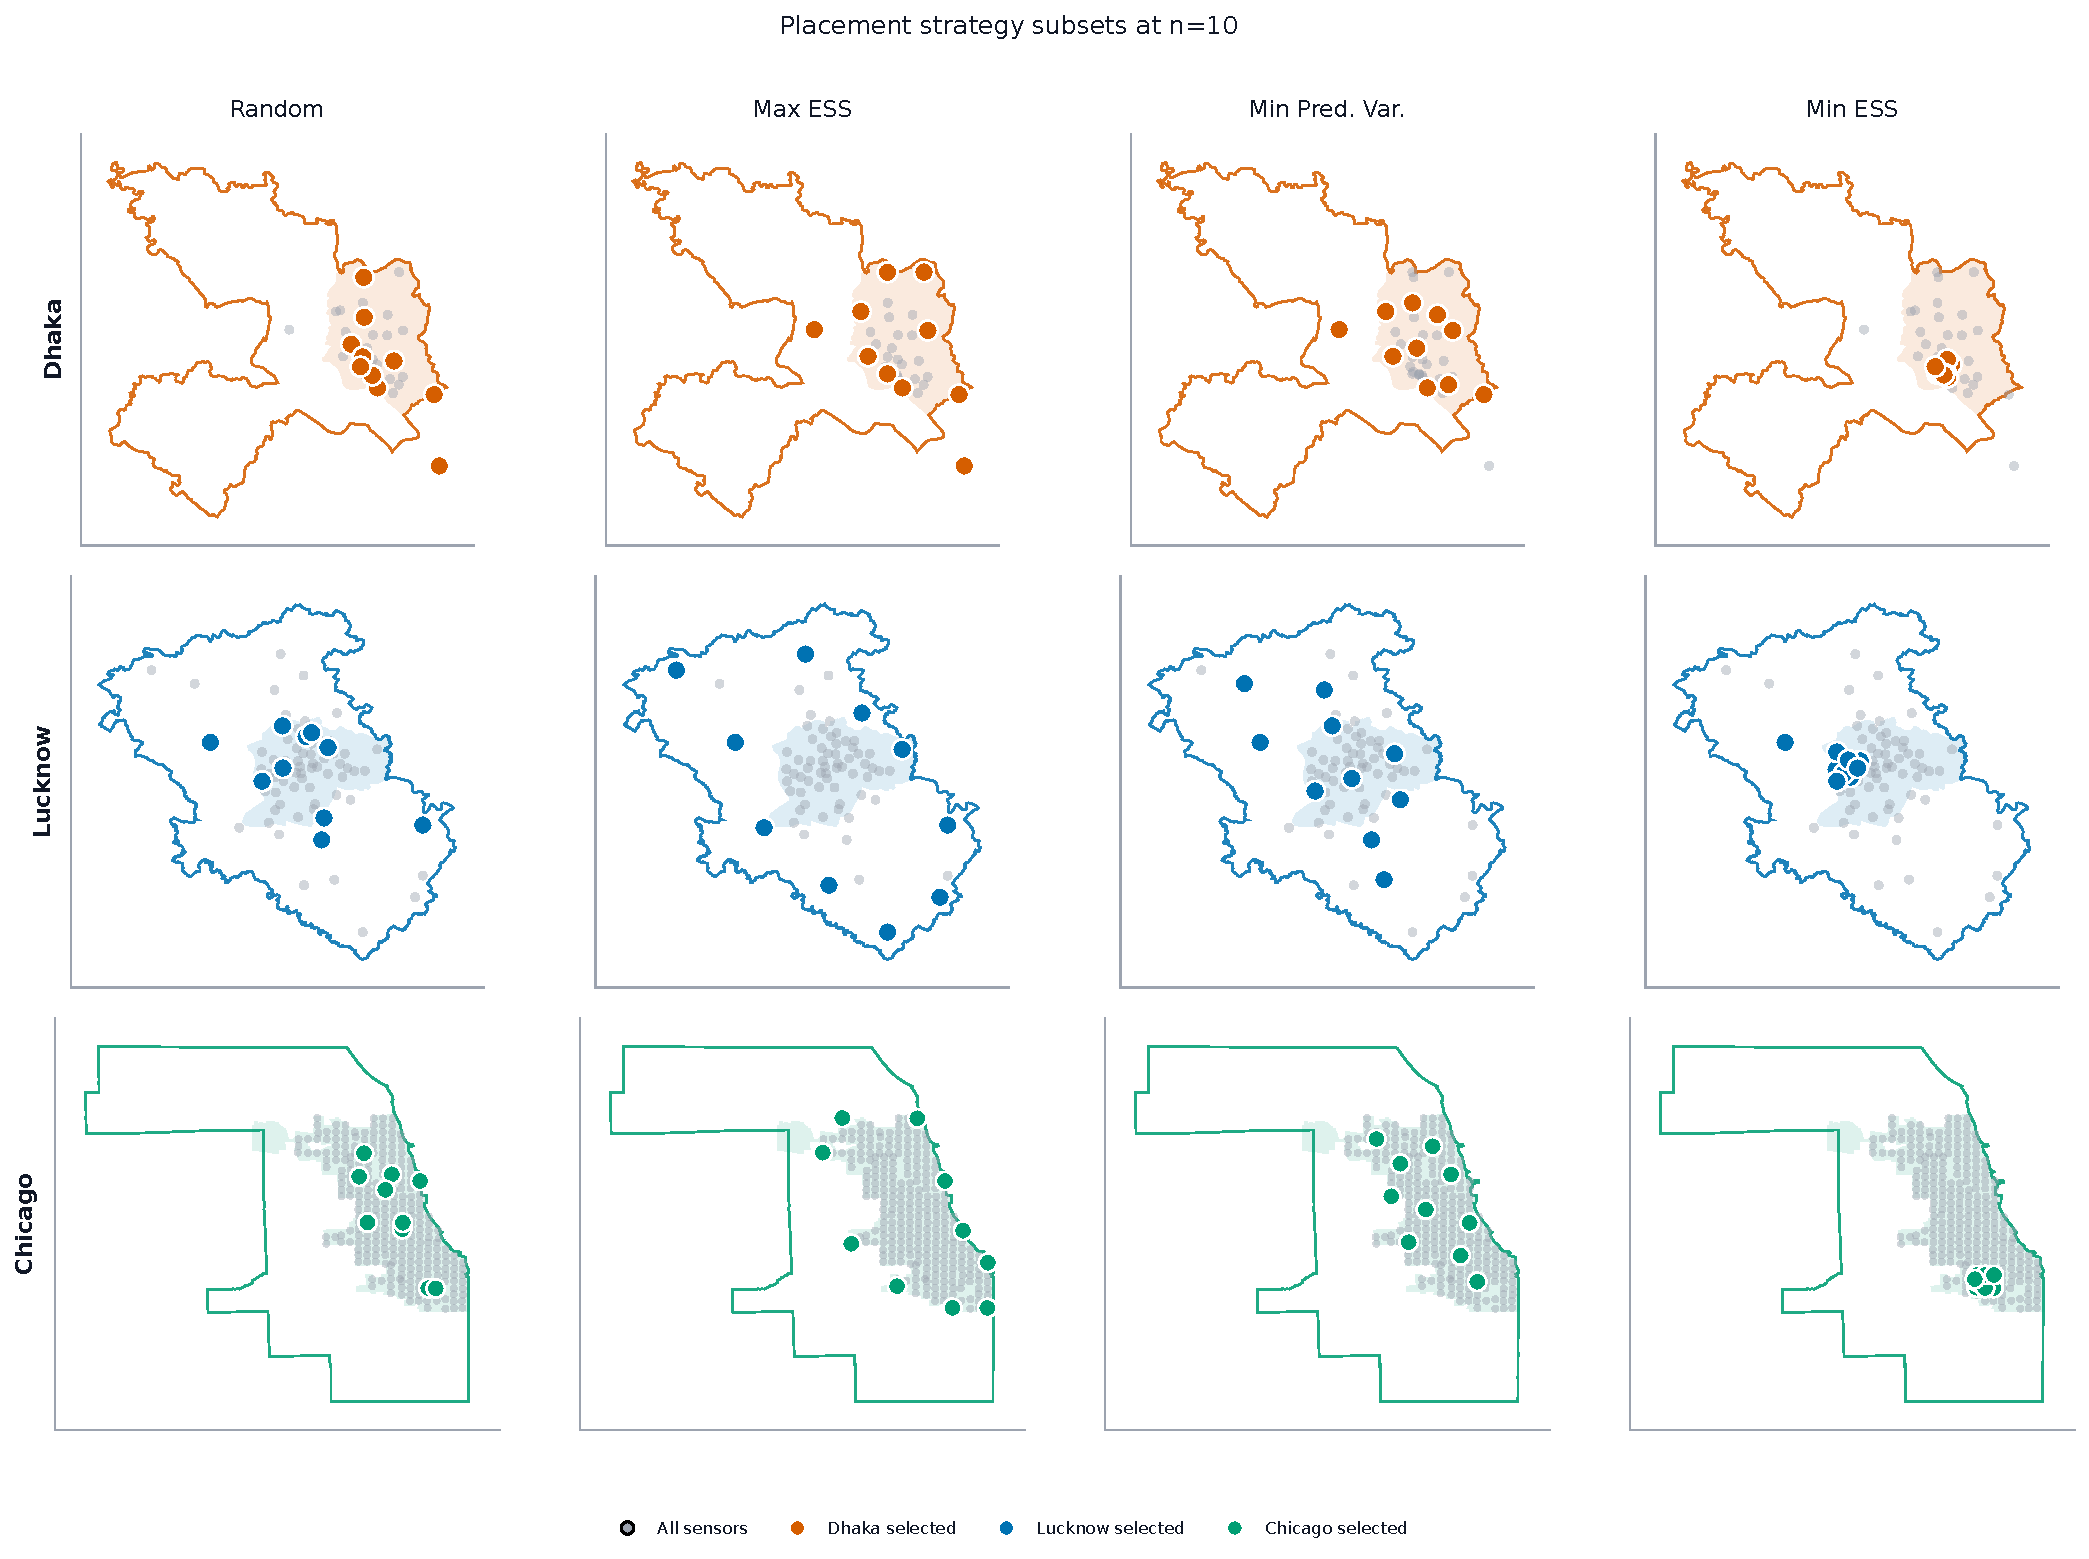
\includegraphics[width=0.98\textwidth]{Plots/Main_text/Figure_4/three_city_placement_strategy_maps_n10.pdf}
    \caption{Example sample locations for $N=10$ under different sampling strategies in \city{Dhaka}, \city{Lucknow}, and \city{Chicago}. All sensors in the networks are shown as gray dots; selected locations are highlighted for deterministic random sampling, maximum effective sample size, minimum predictive variance, and the deliberately clustered minimum-ESS stress test. The maximum-ESS and minimum-predictive-variance designs improve spatial balance relative to a clustered design, with minimum predictive variance favoring coverage of the interior of the area of interest.}
    \label{fig:dhaka_locations}
\end{figure}

This guidance is partly theoretical, given that daily spatial autocorrelation was not consistently detectable in our datasets at the resolvable spacings; the model-based placement criteria therefore rest on the covariance model used in their derivation rather than on directly fitted empirical covariance from these networks. However, consideration of such metrics remains practically useful for ruling out the pathological minimum-ESS case shown in Figure~\ref{fig:dhaka_locations}, where observations are tightly clustered. Such clustering would improve local estimates near the cluster but would not be a defensible estimate of the deployed-network mean \pmtt\ over the broader area of interest. A dual-reference Monte Carlo check that re-evaluates each \city{Chicago} selection strategy against both the selected $N^*=50$ mean and the full $N=277$ mean (Supporting Information~\ref{sec:si_reference_target_sensitivity}) makes this point quantitative: random and k-means stratified selections see at most a $0.07$ percentage-point delta when the reference target switches, whereas cluster-concentrated and anti-cluster selections see $0.33$ and $0.76$ percentage-point penalties.

\subsection{Assumptions and Limitations}\label{sec:assumptions}

All findings in this study rest on two assumptions that we make explicit before discussing limitations in more detail. Our primary estimand is the \emph{deployed-network mean} of the existing deployed sensors, not the true area-weighted or population-weighted pollution field, and not a regulatory compliance metric or an exceedance classification (Figure~\ref{fig:si_estimand_schematic}); sensor-count recommendations should be read against this estimand throughout. The findings are also conditional on the reference networks being well-calibrated, quality-controlled, and reasonably representative of the monitoring target. Under this calibration-sufficiency assumption, and beyond roughly 10--15 well-distributed sensors, improvements in the accuracy of deployed-network mean estimates are more effectively achieved by enhancing calibration fidelity, QA/QC procedures, and maintenance practices than by further increasing node counts. The empirical support for this claim comes from the rapid MdAPE convergence in Figure~\ref{fig:mdape_annual}, combined with the well-documented sensitivity of LCS data to drift, humidity, and environmental cross-sensitivities reported by Bagkis et al.\supercite{bagkis_evolving_2025-1} and others. For resource-constrained deployments, this suggests a design strategy that first secures a modest, spatially representative network and then prioritizes investments in sensor reliability and data quality. By ``properly maintained,'' we mean a network with documented calibration and harmonization against reference-grade monitors with periodic re-calibration, QA/QC screening for sensor faults, drift, and physically implausible values, reasonable temporal completeness with missingness that is not strongly correlated with the analysis target, and operation within ambient PM regimes for which the deployed hardware is rated and characterized.

The primary result of our study is explicitly about how sub-networks perform relative to a larger reference network. The primary estimand is the \emph{reference network mean}, and all performance metrics quantify how well sub-networks of size $n$ reproduce this reference mean and nothing else; we do not target variance or any higher-order features of the reference or sub-networks. This reliance on the reference mean assumes that it is a reasonable approximation of the true value. This assumption is supported by several lines of evidence for the networks in our study. First, both networks are high-fidelity systems with rigorous calibration and harmonization protocols (see Section \ref{sec:qaqc}), including collocation against reference-grade monitors and within-network adjustment factors.\supercite{jain_hybrid_2024,zaman_comparison_2025} Second, the additional diagnostic analysis presented in the Supporting Information (\ref{sec:si_diagnostics}) demonstrates acceptable within-network consistency, broad geographic coverage within the spatial domain of the reference networks and reasonable temporal completeness after QA/QC, summarized using sensor uptime and gap statistics at hourly, daily and annual resolutions. Third, these networks have been used in peer-reviewed studies characterizing seasonal pollution patterns, source contributions, and health impacts in Lucknow and Dhaka, providing independent validation of their representativeness.\supercite{madhwal_evaluation_2024,jain_hybrid_2024,zaman_comparison_2025} Fourth, and perhaps most importantly, the contrasting behaviors observed across cities strengthen confidence in the transferability of our findings. Lucknow's extended spatial footprint ($1{,}505~\mathrm{km}^2$, spanning urban-rural gradients) and Dhaka's compact urban core ($343~\mathrm{km}^2$, high sensor density) represent distinct network geometries and pollution structures, yet both exhibit internally consistent convergence patterns. 

We also require a small set of data-quality assumptions at the methodological level. We assume that networks using this framework are properly calibrated and harmonized at both the sensor-node and network levels, that their measurements are reliable and valid, that QA/QC procedures remove erroneous readings and unreliable nodes, and that any remaining missing data are missing at random and independent of unobserved measurements.

Our spatial analysis assumes first-order stationarity, or that the sensor locations all share the same mean \pmtt\ value. We analyze this assumption in Appendix~\ref{sec:annual_mean_comparison}, finding that this is indeed the case for a majority of the data. This is expected if the majority of \pmtt\ variability may be attributed to seasonal and regional phenomena, and would not be expected if there were consistently localized sources of pollution in the same set of locations. For each city, 2 sensors appeared to have means which were statistically different than the reference mean (at a 95\% Bonferroni-adjusted confidence interval). These sensors had significant missing data during the most polluted parts of the year, which caused their annual mean estimates (and their variance) to be artificially low. Because these sensors represent a small portion of our data, this does not alter our conclusions. However, this raises the point that annual mean estimation on a sensor basis could be improved through imputation or by using the generalized least squares estimate.

Equally important is what we do \emph{not} attempt to do. We do \emph{not} evaluate how well either the reference network or any subnetwork approximates the true pollution field, an area-weighted city mean, a population-weighted exposure mean, or a regulatory-compliance metric defined under specific siting and completeness rules. Any fixed network can only approximate the underlying field, and assessing the gap between the reference network and that field requires independent evidence (e.g., dense satellite retrievals, a much denser short-term colocation campaign, or a process-based chemical transport model) that lies outside the scope of this manuscript. We also do \emph{not} evaluate exceedance classification (whether daily or annual means exceed a stated guideline value) or hotspot detection; both objectives require different analyses, including absolute-concentration thresholds and false-positive / false-negative rates near the threshold.

The findings should also not be assumed to transfer to other PM size fractions. The TSI BlueSky 8143 used in the South Asian networks reports PM\textsubscript{1}, \pmtt, and PM\textsubscript{10} from the same Sensirion SPS30 sensor, but the calibration evidence we cite is specific to \pmtt; the sensor-count guidance reported here should not be applied to PM\textsubscript{1} or PM\textsubscript{10} without separate analysis. Similarly, ambient PM concentration regime matters. Our two South Asian networks operate at concentrations roughly an order of magnitude above the Chicago network, and the partial-year Chicago analysis is included precisely to provide some empirical evidence about transferability to lower-concentration settings; however, we do not have evidence to bound how the sensor-count guidance changes in settings with persistently low concentrations (e.g., remote rural sites) or with substantially different urban form, topography, or source mix.

A further interaction we do not quantify is between network size and calibration quality. Our Monte Carlo isolates the contribution of sampling variability from subnetwork selection; it does not propagate sensor measurement error, calibration drift, humidity artifacts, or correlated errors across sensors into the daily or annual deployed-network mean. A small, well-maintained network may outperform a larger but noisier network for the objective considered here, but our analysis does not formally compare those two regimes (a useful direction for future work).

More broadly, total uncertainty in any deployed-network mean estimate can be viewed as a sum of three components: the within-network subnetwork-sampling error that we quantify directly through the design-based Monte Carlo, a design-uncertainty term arising from incomplete spatial coverage of the deployed network relative to the broader region of interest, and an irreducible measurement-noise floor. At the $n=10$--$20$ subnetwork sizes we recommend, the dominant component is the first; the design-uncertainty term is bounded above by the Chicago finite-population sensitivity and reference-target sensitivity experiments (Supporting Information~\ref{sec:si_finite_population_sensitivity}~and~\ref{sec:si_reference_target_sensitivity}), and a formal decomposition is left to future work.

Regardless of any additional assumptions a reader might wish to impose, the method is formulated for \emph{temporally aggregated means of at least one day}. Our results apply only to the temporal period of the study at aggregation scales of daily or longer; we do not claim validity for sub-daily or real-time metrics. Likewise, our conclusions apply only to the \emph{spatial domain covered by the reference networks} and should not be extrapolated beyond that spatio-temporal support in terms of network-mean replication.

\subsubsection{Practical Recommendations}\label{sec:practical_recommendations}

For networks that are well-calibrated, well-maintained, and spatially distributed across the area of interest, annual deployed-network means can be reproduced to within 5\% typical MdAPE with 10--15 sensors and to within 10\% with as few as 5--7 sensors in our two South Asian networks; daily means require approximately 10 sensors for typical MdAPE $<10\%$ on most days, and 30--40 sensors to satisfy the more conservative expected-error criterion. These counts should be increased when calibration is poorly characterized, when missingness depends on concentration or season, when the target is an area-weighted, population-weighted, or regulatory metric, when sensors are geometrically clustered or source-biased, or when the deployment regime differs materially from the three cities studied here. Neighborhood exposure assessment, exceedance classification near a guideline value, hotspot detection, source attribution, and sub-daily reporting fall outside this scope, and designers with those objectives should treat our numbers as a lower bound. For a municipality with no existing low-cost network, a spatially balanced initial deployment of 10--15 sensors over the area of interest, refined by population density, satellite aerosol optical depth, or emissions inventories as available, provides a defensible starting point.

\subsubsection{Implications for Existing Networks}

The rapid convergence of annual means with as few as 5--7 sensors provides limited but useful retrospective validation for the ``small-$n$'' networks (3--10 nodes) that currently make up nearly half of all documented LCS deployments.\supercite{carotenuto_low-cost_2023} Our results suggest that such small deployments, often dismissed as pilots, can provide informative annual-scale information about a deployed-network mean, but only when the conditions above are met: documented calibration, periodic maintenance, low and non-informative missingness, and spatial distribution across the area of interest. This is a narrower claim than ``robust annual trend data,'' since trend detection is a longitudinal question whose statistical requirements depend on the magnitude of the trend, the year-on-year noise, and the autocorrelation structure of the data, none of which we evaluate here.

Furthermore, the integration deficit between LCS and regulatory frameworks, identified by Carotenuto et al.\ as affecting over 80\% of networks, is partly due to undefined uncertainty.\supercite{carotenuto_low-cost_2023} We use the relative standard error as a simple metric for defining this uncertainty from sufficient statistics, and we show that standard confidence interval calculations have reasonably good coverage above $n \approx 20$. However, the parametric assumptions underlying both uncertainty quantification methods deserve more attention. With agreed-upon standards for LCS uncertainty quantification, the trustworthiness of LCS data for downstream use cases can be improved.

As noted by Bagkis et al., raw LCS data is prone to significant drift and environmental cross-sensitivities.\supercite{bagkis_evolving_2025-1} The redundancy reduction we propose (using fewer sensors) is therefore only viable if the sensors undergo the required calibration and harmonization protocols.


\subsubsection{Future work}
This study presents several opportunities for future work. Normal and lognormal distributional assumptions underlie analyses of coverage and relative standard error; both are clearly too strong on a portion of days. The lack of distributional fit motivates exploration of robust estimators and non-parametric confidence interval definitions, which would support more reliable uncertainty quantification at small $n$.

Several decision-relevant objectives are out of scope here and would each warrant a dedicated analysis. \emph{Threshold and exceedance classification} (whether the network correctly identifies days or years exceeding a stated guideline value) is the most natural extension for public-health-oriented monitoring; the framework would replace MdAPE with classification accuracy, false-positive, and false-negative rates as a function of $n$ and the proximity of the true mean to the threshold. \emph{Area-weighted and population-weighted estimands} would require integrating administrative or census geographies into the aggregation step and would change both the headline numbers and the optimal sensor-placement criterion. \emph{Sub-daily, hotspot, and exposure-gradient} objectives operate at spatial and temporal scales where the daily/annual aggregation used here does not apply; the hourly spatial autocorrelation we report in Supporting Information~\ref{sec:si_hourly_spatial_autocorrelation} suggests these objectives could benefit from spatial estimators. \emph{A formal decomposition of total uncertainty} into the subnetwork-sampling, design (network-coverage), and irreducible measurement-noise components sketched conceptually in Section~\ref{sec:assumptions} would clarify how much of the residual error at moderate $n$ is reducible through additional sensors versus through expanded network coverage or improved instrumentation. Finally, evaluating how calibration quality, siting constraints, and temporal non-stationarity interact with network size across a broader set of cities, pollutants, and concentration regimes would help refine the quantitative thresholds reported here and support more context-specific guidance for low-cost sensor network design.

\section*{References}\addcontentsline{toc}{section}{References} \label{sec:bibliography}
\printbibliography[heading=none]

% Back Matter
\clearpage
\section*{Acknowledgments}
The sensor networks were deployed through the project “Building Capacity to Improve Air Quality in South Asia: Reducing \pmtt\ Through Low-Cost Sensor Network--Driven Policy Decisions” (2020--2025), funded by a grant from the U.S. Department of State. The authors also thank the UL Research Institutes' Chemical Insights for financial support.

\section*{Data Availability}
\label{app:data}
Upon acceptance, data and code will be made available through the Duke Digital Repository, where the release will be assigned a persistent DOI. The release will include the processed hourly and daily \pmtt\ matrices for each network, the sensor location metadata, the Monte Carlo sampling and summary scripts used to generate the main and supporting figures, and the analysis scripts and retained result outputs used to produce the diagnostic outputs cited in the Supporting Information.

\section*{Supporting Information}\label{sec:SI_details}
The Supporting Information contains the following sections that further support the paper.

\begin{itemize}
  \item \textbf{\secref{sec:si_diagnostics}}: post-QA/QC diagnostics for all three networks, including uptime and completeness summaries, the daily $N^*$ distribution, missingness-vs-concentration and missingness-vs-spatial-variability screens, completeness-threshold sensitivity analyses, low-but-nonzero outlier diagnostics, a diurnal-feature preservation check at $n \in \{5, 10, 20\}$, the Chicago network description, an LCS-vs-AQS instrument comparison, and a Chicago raw-vs-calibrated sensitivity analysis. These diagnostics support the finite-population framing used in \nameref{sec:methods} and \Cref{sec:monte_carlo}.
  \item \textbf{\secref{sec:si_metrics}}: formal definitions of APE/MdAPE, absolute concentration error, RSE, and quantile coverage error, plus a compact metric-to-question mapping and discussion of distributional considerations used in the uncertainty and error metrics (\Cref{sec:estimators_metrics}).
  \item \textbf{\secref{sec:si_spatial_diagnostics}}: pairwise-distance diagnostics and Moran's $I$ tests, with distance-band sensitivity (2~km, 5~km, 10~km, and adaptive nearest-neighbor weights) and a variogram/correlogram analysis. These support the conclusion that daily spatial dependence is not consistently detectable at the resolvable spacings of these networks (\Cref{sec:analytical_considerations} and Discussion).
  \item \textbf{\secref{sec:si_estimators}}: derivations and intuition for GLS/ESS and block-kriging (minimum predictive variance) objectives, illustrative sampling configurations, and an empirical comparison of subnetwork performance under random, spatially balanced, max-ESS, and min-predictive-variance placement strategies, supporting the sensor-placement discussion (\Cref{sec:placement} and \Cref{sec:assumptions}).
  \item \textbf{\secref{sec:si_model_based}}: Shapiro--Wilk distributional test summaries and RSE-based sample-size calculations (normal vs.\ lognormal; standard vs.\ robust), including exceedance-style plots referenced in the Discussion.
  \item \textbf{\secref{sec:si_design_based}}: additional Monte Carlo summaries (relative bias, quantile coverage error, 75th/90th/95th APE percentiles for worst-case characterization, absolute-concentration error figures, high-error-day characterization, and seasonal/monthly subnetwork convergence) that complement the main-text estimator-performance discussion (\Cref{sec:bias_coverage}).
  \item \textbf{\secref{sec:annual_mean_comparison}}: comparison of annual mean uncertainty on a sensor basis, to determine whether sensor-level means are statistically distinguishable from the reference mean after temporal autocorrelation adjustment.
\end{itemize}
% --- Table of Contents (graphical abstract) ---
\begin{center}
\textit{Graphical Table of Contents / Picture Abstract}\\[2pt]
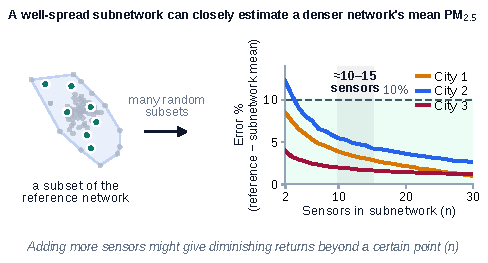
\includegraphics[width=11.25cm]{Plots/TOC/TOC_v2.pdf}
\end{center}
\clearpage
\begin{refsection}
\appendix
\subfile{appendix/appendix}
\end{refsection}

\end{document}
